\chapter{Trees}

\tikzset{vtx/.style={circle,fill=black,inner sep=1.6pt}}

Trees are the minimal connected graphs. They appear everywhere (search trees, spanning
networks, parse trees) and their simple structure makes them the base case of many proofs.

\section{Definitions and basic properties}

\begin{definition}[Tree, forest, leaf]
A \emph{tree} is a connected graph with no cycles. A \emph{forest} is a graph with no cycles
(so each component is a tree). A \emph{leaf} is a vertex of degree $1$.
\end{definition}

\begin{center}
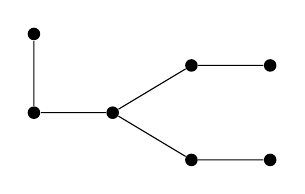
\begin{tikzpicture}
  \node[vtx] (a) at (0,0) {};
  \node[vtx] (b) at (1,0) {};
  \node[vtx] (c) at (2,0.6) {};
  \node[vtx] (d) at (2,-0.6) {};
  \node[vtx] (e) at (3,0.6) {};
  \node[vtx] (f) at (0,1) {};
  \node[vtx] (g) at (3,-0.6) {};
  \draw (a)--(b)--(c)--(e) (b)--(d)--(g) (a)--(f);
\end{tikzpicture}
\end{center}

\begin{lemma}
In a tree, there is a unique path between any two vertices.
\end{lemma}
\begin{proof}
A path exists by connectedness. If $P \ne P'$ were two paths from $u$ to $v$, follow them from
$u$ until they first diverge, at vertex $x$, and let $y$ be the next vertex after $x$ on $P$
that also lies on $P'$ (it exists since both end at $v$). The parts of $P$ and $P'$ between $x$
and $y$ form a cycle, a contradiction.
\end{proof}

\begin{lemma}
Every edge of a tree is a bridge.
\end{lemma}
\begin{proof}
An edge is a bridge iff it lies on no cycle, and a tree has no cycles.
\end{proof}

\begin{theorem}
A tree with $p$ vertices has exactly $p - 1$ edges.
\end{theorem}
\begin{proof}
Induction on $p$. For $p = 1$ there are no edges. For $p \ge 2$, a tree $T$ has an edge $e$,
which is a bridge, so $T - e$ has exactly two components $T_1, T_2$, each connected with no
cycles, i.e.\ trees, with $p_1 + p_2 = p$ vertices and $p_1, p_2 < p$. By induction
$\abs{E(T)} = (p_1 - 1) + (p_2 - 1) + 1 = p - 1$.
\end{proof}

\begin{corollary}
A forest with $p$ vertices and $c$ components has $p - c$ edges.
\end{corollary}

\begin{theorem}
Every tree with at least $2$ vertices has at least $2$ leaves.
\end{theorem}
\begin{proof}
Take a longest path $v_0v_1\cdots v_k$ ($k \ge 1$). Any neighbour of $v_k$ other than $v_{k-1}$
would either extend the path (if off the path) or close a cycle (if on it); neither is possible,
so $\deg(v_k) = 1$. Similarly $\deg(v_0) = 1$.
\end{proof}

\begin{aside}
A sharper count: if $n_i$ is the number of vertices of degree $i$ in a tree with at least
$2$ vertices, then $n_1 = 2 + \sum_{i\ge3}(i-2)n_i$. This follows from the handshake lemma:
$\sum_i i\,n_i = 2(p-1) = 2\sum_i n_i - 2$, so $\sum_i (i-2)n_i = -2$. For example, a tree with
two vertices of degree $3$ and one of degree $4$ has $2 + 2 + 2 = 6$ leaves.
\end{aside}

\begin{theorem}[Characterizations of trees]
For a graph $G$ with $p$ vertices, any two of the following imply the third:
(a) $G$ is connected; (b) $G$ has no cycles; (c) $G$ has $p-1$ edges.
\end{theorem}
\begin{proof}
(a)+(b)$\Rightarrow$(c) is the theorem above. (b)+(c)$\Rightarrow$(a): $G$ is a forest with
$p - c$ edges, so $c = 1$. (a)+(c)$\Rightarrow$(b): if $G$ had a cycle, delete an edge on it; the
result is still connected (the edge was not a bridge). Repeat until no cycles remain; we get a
tree with $p$ vertices and fewer than $p - 1$ edges, a contradiction.
\end{proof}

Equivalently: $G$ is a tree iff it is minimally connected (connected, and every edge is a bridge)
iff it is maximally acyclic (no cycle, but adding any edge creates one).

\section{Spanning trees}

\begin{definition}[Spanning tree]
A \emph{spanning tree} of $G$ is a spanning subgraph of $G$ that is a tree.
\end{definition}

\begin{theorem}
$G$ is connected if and only if $G$ has a spanning tree.
\end{theorem}
\begin{proof}
If $G$ has a spanning tree $T$, any two vertices are joined by a path in $T \subseteq G$.
Conversely, if $G$ is connected, repeatedly delete an edge lying on a cycle. Such edges are not
bridges, so connectivity is preserved; the process stops with a connected acyclic spanning
subgraph.
\end{proof}

\begin{corollary}
A connected graph with $p$ vertices has at least $p - 1$ edges.
\end{corollary}

\begin{lemma}
Let $T$ be a spanning tree of $G$ and $e \in E(G) \setminus E(T)$.
\begin{enumerate}
  \item $T + e$ contains exactly one cycle.
  \item If $f$ is an edge on that cycle, then $T + e - f$ is again a spanning tree.
\end{enumerate}
\end{lemma}
\begin{proof}
(1) If $e = uv$, cycles of $T + e$ must use $e$, and correspond to paths from $u$ to $v$ in $T$,
of which there is exactly one. (2) $T + e - f$ is connected ($f$ lies on a cycle so is not a
bridge of $T + e$) and has $p - 1$ edges, so it is a tree.
\end{proof}

\section{Breadth-first search}

Breadth-first search (BFS) finds a spanning tree of a connected graph, and in fact decides
connectivity in general.

\begin{important}[BFS]
Choose a root $r$; set $\mathrm{level}(r) = 0$ and put $r$ in a queue. Repeatedly take the
vertex $v$ at the front of the queue; for each neighbour $w$ of $v$ not yet seen, mark it seen,
set $\mathrm{pr}(w) = v$ (its parent), $\mathrm{level}(w) = \mathrm{level}(v) + 1$, and append
$w$ to the queue. Stop when the queue is empty.
\end{important}

The edges $w\,\mathrm{pr}(w)$ form a tree (each new vertex adds one edge to one new vertex)
spanning the component of $r$. If some vertex is never seen, $G$ is disconnected, and the set
of seen vertices $X$ has $\delta(X) = \emptyset$.

\begin{theorem}
In a BFS tree of a connected graph $G$, the level of $v$ is the distance from $r$ to $v$, and for
every edge $uv$ of $G$ (tree edge or not), $\abs{\mathrm{level}(u) - \mathrm{level}(v)} \le 1$.
\end{theorem}
\begin{proof}[Proof sketch]
Vertices leave the queue in non-decreasing order of level. If $u$ is processed before $v$ and
$uv$ is an edge, then when $u$ is processed either $v$ is already seen (with level at most
$\mathrm{level}(u) + 1$, and at least $\mathrm{level}(u)$ since it comes later) or $v$ gets level
$\mathrm{level}(u) + 1$.
\end{proof}

\section{Odd cycles and bipartite graphs}

\begin{theorem}
A graph is bipartite if and only if it has no odd cycle.
\end{theorem}
\begin{proof}
We already know odd cycles are not bipartite, so a bipartite graph contains none.

Conversely, suppose $G$ has no odd cycle. It suffices to treat each component separately, so let
$G$ be connected, and take a BFS tree with root $r$. Let $X$ be the vertices of even level and $Y$
those of odd level. Suppose some edge $uv$ has both ends in $X$ or both in $Y$; by the theorem
above, $\mathrm{level}(u) = \mathrm{level}(v)$. Let $w$ be the last common vertex of the tree paths
from $r$ to $u$ and to $v$. The tree paths from $w$ to $u$ and from $w$ to $v$ have the same
length $\ell$, and together with $uv$ they form a cycle of length $2\ell + 1$, which is odd. This
contradiction shows $(X,Y)$ is a bipartition.
\end{proof}

So bipartiteness can be checked efficiently, and either way BFS produces a certificate: a
bipartition, or an odd cycle.

\section{Minimum spanning trees}

Suppose each edge $e$ has a cost $w(e)$. A \emph{minimum spanning tree} (MST) is a spanning tree
of minimum total cost.

\begin{important}[Prim's algorithm]
Start with $T$ containing a single vertex. While $T$ does not span $G$, among the edges with
exactly one end in $T$ (the cut $\delta(V(T))$), add a cheapest one to $T$.
\end{important}

\begin{theorem}
Prim's algorithm returns a minimum spanning tree of a connected graph.
\end{theorem}
\begin{proof}[Proof sketch]
We show by induction that after each step, $T$ is contained in some MST $T^*$. Suppose this holds,
and the algorithm adds $e$, a cheapest edge of $\delta(V(T))$. If $e\in T^*$ we are done.
Otherwise $T^* + e$ has a unique cycle, which crosses the cut $\delta(V(T))$ at $e$ and so must
cross it again at some edge $f \neq e$. Then $T^* + e - f$ is a spanning tree with cost
$w(T^*) + w(e) - w(f) \le w(T^*)$ since $w(e)\le w(f)$; so it is also an MST, and it contains
$T + e$.
\end{proof}

\begin{example}
Vertices $a,b,c,d$ with costs $ab = 1$, $bc = 2$, $ac = 3$, $cd = 4$, $bd = 5$. Starting at $a$:
add $ab$ ($1$), then the cheapest edge leaving $\{a,b\}$ is $bc$ ($2$), then leaving $\{a,b,c\}$ is
$cd$ ($4$). The MST $\{ab,bc,cd\}$ has cost $7$.
\end{example}

\section{Summary}
\begin{itemize}
  \item Tree: connected, acyclic; unique paths; every edge a bridge; $p - 1$ edges; at least two leaves.
  \item Any two of connected / acyclic / $p-1$ edges imply the third.
  \item Connected iff a spanning tree exists; $T + e$ has one cycle and $T + e - f$ is a spanning tree.
  \item BFS: levels are distances; non-tree edges join levels differing by at most $1$.
  \item Bipartite iff no odd cycles. Prim's algorithm finds an MST.
\end{itemize}
